\documentclass[a4paper, 10pt]{article}

\usepackage{../packages}

\graphicspath{{./figures}}


\begin{document}
\begin{titlepage}
\begin{center}
	
\includegraphics[scale=0.7]{logo.png}

	\vspace*{4cm}
	\textbf{Bazy danych\\ Laboratorium}

	\vspace{1.5cm}
	\textit{Zarządzanie bazą danych Oracle}

	\vspace{1.5cm}
	\textbf{Stanislau Antanovich}\\
	nr. indeksu: 173590\\
	gr. lab: L04

	\vspace{4.5cm}
	%\today
\end{center}
\end{titlepage}

\tableofcontents
\listoffigures
\lstlistoflistings

\newpage

\section{Realizacja}

\begin{enumerate}
	\item Tworzenie przestrzeni TABLESPACE o nazwie ``\emph{project\_tablespace}''.
		\begin{lstlisting}[style=SQL, caption=\textit{Tworzenie przestrzeni TABLESPACE o nazwie ``project\_tablespace''}]
CREATE TABLE SPACE project_tablespace
DATAFILE 'project_tablespace.dbf' SIZE 100M
AUTOEXTEND ON NEXT 10M MAXSIZE UNLIMITED;
		\end{lstlisting}
		\begin{figure}[H]
			\centering
			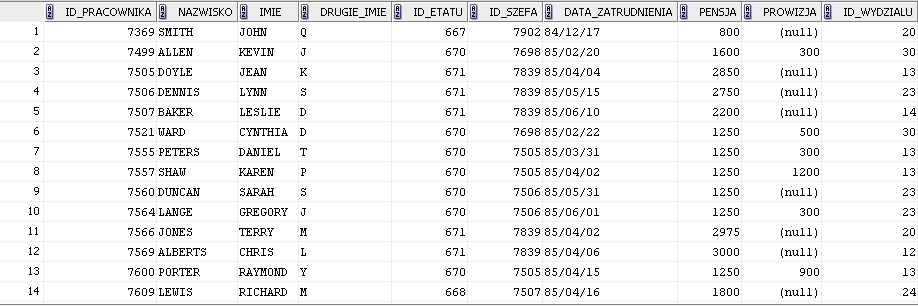
\includegraphics{zadanie1.png}
			\caption{\textit{Tworzenie przestrzeni TABLESPACE o nazwie ``project\_tablespace''}}
		\end{figure}
	\item Tworzenie używtkownika dla nowej bazy danych oraz przestrzeni o danych:
		\begin{itemize}
			\item nazwa: ``student1''
			\item hasło: zgodnym z dniem tworzenia np. ``07052023''
		\end{itemize}
		Przypisanie do konta użytwkownika przestrzeń ``\emph{project\_tablespace}'' oraz odpowiednie dostępy oraz role.
		\begin{lstlisting}[style=SQL, caption=\textit{Tworzenie użytkownika}]
		\end{lstlisting}
		\begin{figure}[H]
			\centering
			%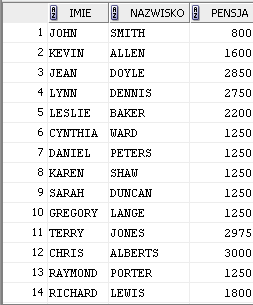
\includegraphics{zadanie2.png}
			\caption{\textit{Tworzenie użytwkonika}}
		\end{figure}
	\item Wdrożenie bazy danych. 
		\begin{lstlisting}[style=SQL, caption=\textit{Wdrożenie bazy danych}]
		\end{lstlisting}
		\begin{figure}[H]
			\centering
			%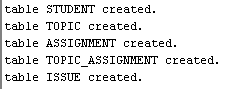
\includegraphics{zadanie3.png}
			\caption{\textit{Wdrożenie bazy danych}}
		\end{figure}
	\item Tworzenie sekwencji ``\emph{student\_seq}'' dedykowaną dla studenta w przedziale od 0 do 10000.
		\begin{lstlisting}[style=SQL, caption=\textit{Tworzenie sekwencji ``student\_seq''}]
		\end{lstlisting}
		\begin{figure}[H]
			\centering
			%
\includegraphics{zadanie4.png}
			\caption{\textit{Tworzenie sekwencji ``student\_seq''}}
		\end{figure}
	\item Funkcja, która pozwala dodać nowego studenta (addStudent). Wykorzystanie utworzonej sekwencji ``\emph{student\_seq}'' dla ustalenia kolejnego ID. Zwracanie z funkcji ID dodanego studenta.
		\begin{lstlisting}[style=SQL, caption=\textit{Funkcja, która dodaje nowego studenta}]
		\end{lstlisting}
		\begin{figure}[H]
			\centering
			%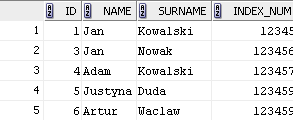
\includegraphics{zadanie5.png}
			\caption{\textit{Funkcja, która dodaje nowego studenta}}
		\end{figure}
	\item Wprowadzenie danych do tablicy. Wywołanie funkcji addStudent.
		\begin{lstlisting}[style=SQL, caption=\textit{Wprowadzenie danych do tablicy}]
		\end{lstlisting}
		\begin{figure}[H]
			\centering
			%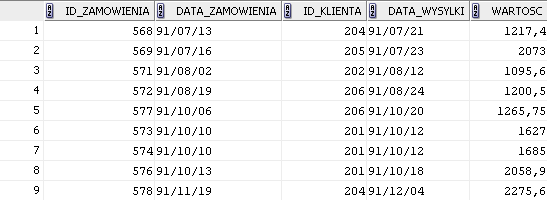
\includegraphics{zadanie6.png}
			\caption{\textit{Wprowadzenie danych do tablicy}}
		\end{figure}
	\item Tworzenie widoków odpowiedzialnych za:
		\begin{itemize}
			\item wyświetlenie wszystkich tematów projektów 
			\item wyświetlenie wszystkich studentów, którzy nie mają przypisanego tematu
		\end{itemize}
		\begin{lstlisting}[style=SQL, caption=\textit{Tworzenie widoków}]
		\end{lstlisting}
		\begin{figure}[H]
			\centering
			%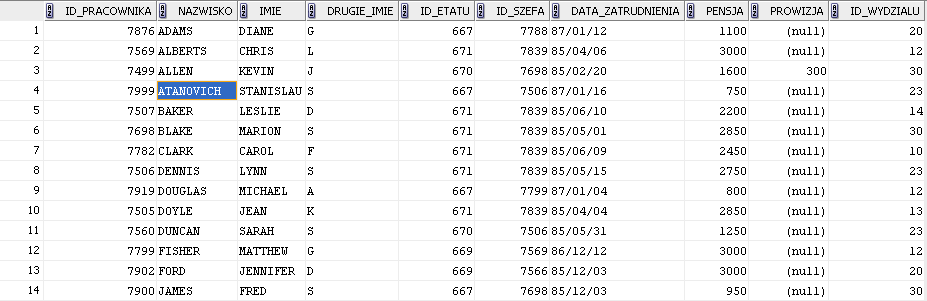
\includegraphics{zadanie7.png}
			\caption{\textit{Tworzenie widoków}}
		\end{figure}
	\item Zwracanie raportu do pliku o rozszerzeniu \emph{.csv} z informacją o nagłówku(kolumny):
		\begin{itemize}
			\item dane studenta(indeks, imię oraz nazwisko), nazwa projektu, ocena
			\item zwracanie danych osób, które uzyskały pozytywną ocenę(większą lub równą niż 3.0)
		\end{itemize}
		\begin{lstlisting}[style=SQL, caption=\textit{Zwracanie raportu do pliku}]
		\end{lstlisting}
		\begin{figure}[H]
			\centering
			%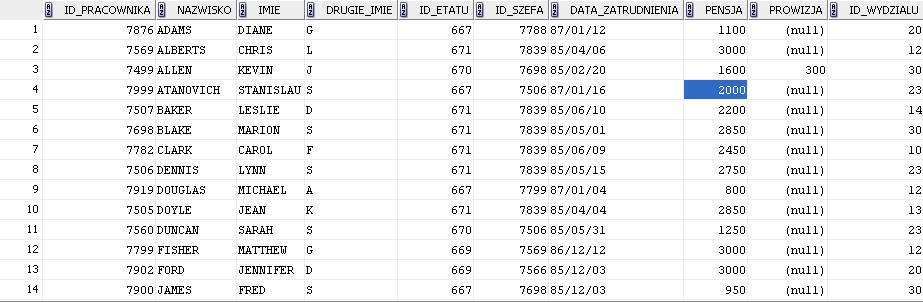
\includegraphics{zadanie8.png}
			\caption{\textit{Zwracanie raportu do pliku}}
		\end{figure}
\end{enumerate}

\section{Wnioski}
Dzieki dzialaniom wykonanym podczas laboratorium udalo sie poszerzyć wiedze na temat baz danych oraz zrozumieć, jakie możliwości oferuja. Pozwolilo to nie tylko na zdobycie teoretycznej wiedzy, ale również na praktyczne zastosowanie różnych funkcji SQL w rzeczywistych scenariuszach.

\end{document}
